\chapter{Background}

Questo capitolo intende esporre i concetti principali per una corretta comprensione della presente tesi, introducendo dapprima le blockchain, mostrando la prima realizzazione di blockchain, ovvero Bitcoin, ed infine introducendo le strutture dati autenticate e le Distributed Hash Table.


\section{DLT e Blockchain}\label{sec:blockchain}

Un \emph{Distributed Ledger Technology}, o \emph{DLT}, è un registro distribuito, la cui copia è presente su tutti i partecipanti (o nodi) della rete, in cui ogni nodo in maniera indipendente dagli altri può apportare delle modifiche sotto il consenso di tutti gli altri. Ogni nodo della rete è in grado di creare una transazione che modifica lo stato del registro, ma questa non è accettata da un'autorità centralizzata come in sistemi tradizionali, bensì dalla maggioranza dei partecipanti. Infatti, ogni nodo può partecipare alla validazione e alla conferma di tutte le nuove transazioni.

Il concetto fondamentale che regola una DLT è quello del \emph{consenso}. Il consenso specifica come i partecipanti si accordano sullo stato del registro. Quest'ultimo, oltre ad essere distribuito, è anche \emph{immutabile}. Infatti, una volta raggiunto il consenso su una transazione, questa non può essere annullata ed il suo effetto rimane indelebile.

Le DLT si dividono in due categorie: \emph{permissioned} (o \emph{private}) e \emph{unpermissioned} (o \emph{pubbliche}). Nelle prime l'accesso è controllato da un'autorità che verifica l'autenticità del partecipante, il registro è quindi proprietà di un insieme di attori, ed il sistema è composto da nodi fidati (\emph{trusted}). Le seconde, argomento della presente tesi, permettono a chiunque di partecipare, non sono quindi proprietà di nessuna organizzazione e consentono a tutti di proporre delle modifiche. Il campo di applicazione è quello di database su scala globale, ad esempio per un sistema di cripto-valute, le cui informazioni hanno bisogno di essere immutabili (le transazioni confermate o il saldo associato ai conti degli utenti). Esse sono però soggette ad attacchi Sybil~\cite{douceur2002sybil}, di cui si parlerà in seguito. In genere le prestazioni delle DLT permissioned sono maggiori delle DLT unpermissioned. Nel resto della tesi si farà riferimento solamente alle DLT unpermissioned.

Poiché i database tradizionali hanno un failure model nettamente differente da quello delle DLT, i protocolli di consenso utilizzati nei primi in ambiente distribuito, come~\cite{bernstein1987concurrency, raz1995dynamic}, non possono essere impiegati. Infatti, mentre nei database il fallimento di un nodo corrisponde ad un suo crash, software o hardware, che non gli permette di rispondere alla richieste, nelle seconde l'ambiente di esecuzione è più ostile. I nodi, denominati \emph{bizantini}, oltre ad avere dei crash, possono comportarsi in modo malevolo, rispondendo in modo errato e corrompendo altri nodi.
Le DLT devono quindi adottare un protocollo di consenso che sia \emph{Byzantine Fault Tollerant} (\emph{BFT}), il cui nome deriva dal \textit{problema dei generali bizantini}.
\textit{Proof-of-Work}~\cite{nakamoto2019bitcoin}, in cui si seleziona randomicamente un leader la cui probabilità dipende dalla sua potenza computazionale, \textit{Proof-of-Stake}~\cite{kiayias2017ouroboros}, \textit{Proof-of-Personhood}~\cite{borge2017proof}, sono esempi di protocolli BFT resistenti ad attacchi Sybil.

Una \emph{blockchain} fa parte della classe delle DLT ed è una lista di blocchi semplicemente collegata, il cui inserimento è solo in modalità \emph{append}. Ogni blocco è identificato da un hash crittografico, calcolato sull'header del blocco stesso. Ogni blocco punta al nodo precedente specificandone l'hash. La sequenza di blocchi crea quindi una catena, in cui il primo è denominato \emph{genesis block} ed è specificato nell'algoritmo di consenso.

In Bitcoin~\cite{nakamoto2019bitcoin}, un blocco è un contenitore formato da una sezione \textit{metadati}, composto dalla dimensione del blocco stesso, da un \textit{block header} di 80 byte e dalla lista di transazioni validate. Il block header è composto dall'hash del precedente blocco, dal \emph{root-hash} del Merkle Tree formato dalle transazioni contenute nel blocco, un \emph{timestamp}, ovvero il tempo di creazione del blocco, un \emph{difficulty target} e un \emph{nounce}, utilizzati nella fase di mining.
La figura~\ref{fig:bitcoin_blockchain} mostra un esempio di blockchain.

\begin{figure}
	\centering
	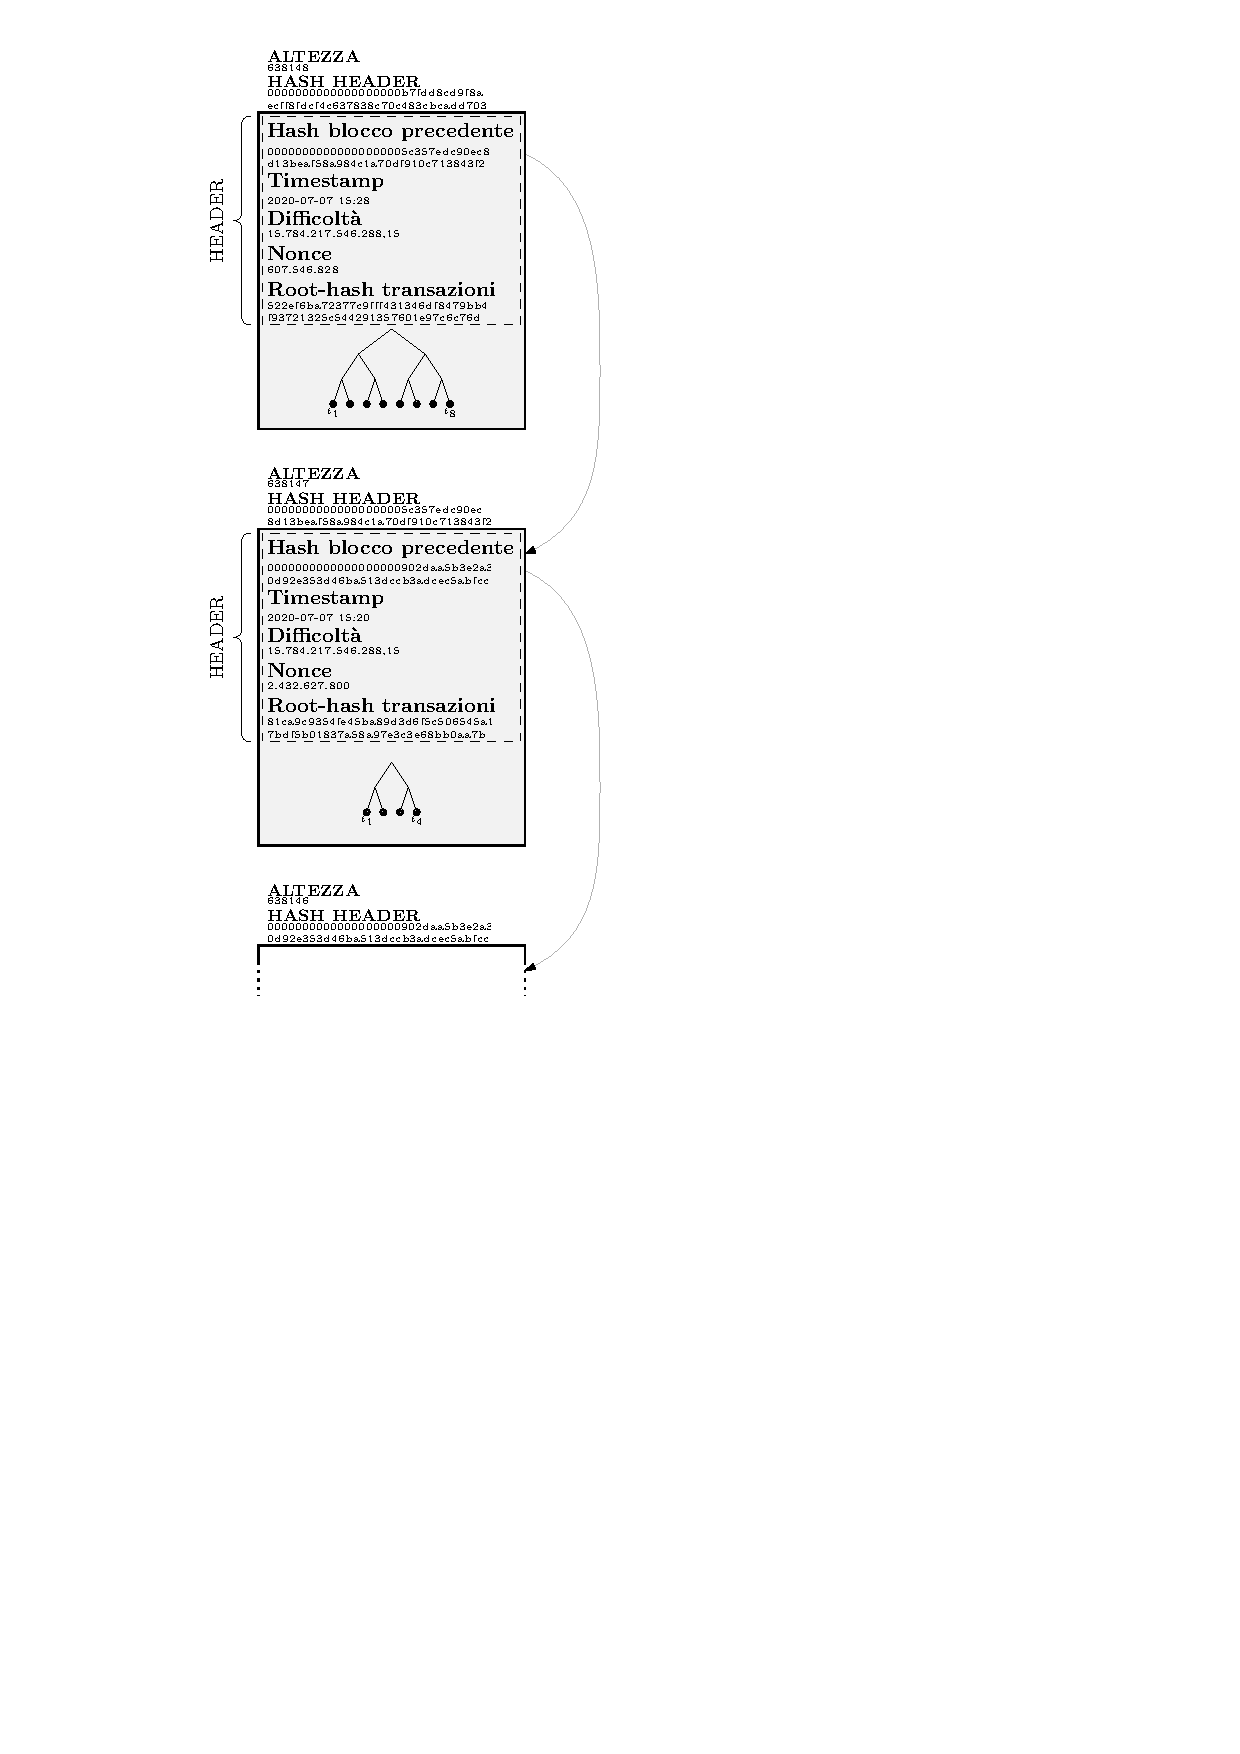
\includegraphics{img/capuno/blockchain_bitcoin.pdf}
	\caption{Esempio di blockchain in Bitcoin. Ogni blocco punta al blocco precedente specificandone l'hash dell'header.}
	\label{fig:bitcoin_blockchain}
\end{figure}


\section{Bitcoin}
Bitcoin~\cite{nakamoto2019bitcoin} è una tecnologia open-source di cripto-valute basata su blockchain, presentato nel 2008 da Satoshi Nakamoto, la cui identità è ancora un mistero.
A differenza di valute tradizionali che esistono fisicamente sotto forma di banconote, il \textit{bitcoin}, la valuta dell'omonima tecnologia, è virtuale. Con il termine Bitcoin, si indicano vari aspetti: la tecnologia, lo stack protocollare di comunicazione adottato tra i partecipanti alla rete e la valuta scambiata.
Bitcoin è una rete P2P, a cui partecipano nodi denominati \emph{peer}, in cui non esistono nodi speciali o più importanti di altri, come nei sistemi di pagamento elettronici tradizionali. Non è presente quindi un server centrale che gestisce tutti i pagamenti.

Il concetto fondamentale di Bitcoin è quello di \emph{transazione}. Una transazione trasferisce dei bitcoin da una conto sorgente ad un conto destinazione. Ogni peer può creare una transazione, dimostrando di essere il proprietario del conto sorgente. Dopo la creazione, questa viene inviata in broadcast a tutti i nodi della rete, per essere validata. A differenza dei sistemi di pagamento elettronici tradizionali, in cui un server centrale accetta o rifiuta le transazioni generate dai propri clienti, le transazioni sono accettate o rifiutate dalla rete Bitcoin secondo un meccanismo di \emph{consenso distribuito}, utilizzando un approccio denominato \emph{Proof-of-Work}. Le transazioni accettate vengono raggruppate in blocchi di transazioni, secondo un processo che richiede un enorme quantità di potenza computazionale. Al termine di questa fase il blocco viene aggiunto in \emph{blockchain}. Questo processo è denominato \emph{mining} ed è svolto dai peer che ricoprono il ruolo di \emph{miner}. Il mining ha due obiettivi:
\begin{enumerate}
	\item creazione di bitcoin: ogni nodo che aggiunge un blocco alla blockchain viene ricompensato dalla rete con una quantità di bitcoin fissata per ogni blocco e che decresce nel tempo;
	\item validazione delle transazioni secondo le regole di consenso, assicurando che esse siano valide.
\end{enumerate}
Una transazione è valida se è corretta sintatticamente e non fa \textit{double-spending}, ovvero spende due o più volte lo stesso importo.
 
Inizialmente il mining veniva effettuato da personal computer potenti. Man mano che i miner si aggiungevano alla rete Bitcoin, per cui diveniva sempre più difficile \emph{minare} un blocco, si utilizzarono delle Graphical Processing Units, o GPU, come quelle utilizzate nei videogiochi. Tuttavia negli ultimi anni, a causa dell'elevato numero di miner presenti sulla rete, si utilizzano sistemi Application Specific Integrated Circuit, o ASIC, che implementano in hardware gli algoritmi di mining impiegati in Bitcoin per aumentare le performance. Sono state create anche soluzioni che hanno l'obiettivo di condividere la propria potenza computazionale in \textit{mining pool}, composte da diversi partecipanti, che dividono equamente, sulla base delle risorse condivise, i bitcoin guadagnati.

\subsection{Wallet e indirizzi digitali}
Un nodo, per poter partecipare alla rete ed effettuare un pagamento, ha bisogno di una \emph{chiave digitale} e di un \emph{bitcoin address}. Un utente può generare un numero qualsiasi di chiavi digitali, che vengono memorizzate in un database locale, denominato \emph{wallet}.
La possibilità di generate autonomamente delle chiavi evidenzia la caratteristica fondamentale di Bitcoin, ovvero la decentralizzazione del controllo e del consenso, basate sulla crittografia.
In particolare, il modello di riferimento è quello della crittografia asimmetrica, in cui le chiavi digitali sono sotto forma di una coppia di chiavi, una \emph{privata} (e segreta), ed una \emph{pubblica}, che deriva dalla chiave privata. \'E importante specificare che l'uso della crittografia non ha uno scopo di \emph{confidenzialità}, d'altronde tutto in Bitcoin viaggia in chiaro, ma per \emph{autenticità}, per dimostrare di essere possessori di un certo conto.
In crittografia, una chiave privata è usata per firmare un messaggio, o in questo caso una transazione, mentre la chiave pubblica, conosciuta da tutti i nodi della rete, per validare la firma del messaggio. Infatti, semplificando, la chiave pubblica è usata per ricevere i bitcoin, mentre la chiave privata per spenderli, secondo delle modalità che saranno note nel proseguimento della lettura dei prossimi paragrafi, in cui si mostra la creazione di una transazione da parte di un peer, e quindi le prove crittografiche che deve mostrare in modo da poter spendere i suoi bitcoin.
In una transazione, l'indirizzo di destinazione è indicato da un \emph{bitcoin address}, che deriva dalla chiave pubblica del peer, mediante una serie di funzioni hash, come illustrato nella Figura~\ref{fig:bit_address}.

\begin{figure}
	\centering
	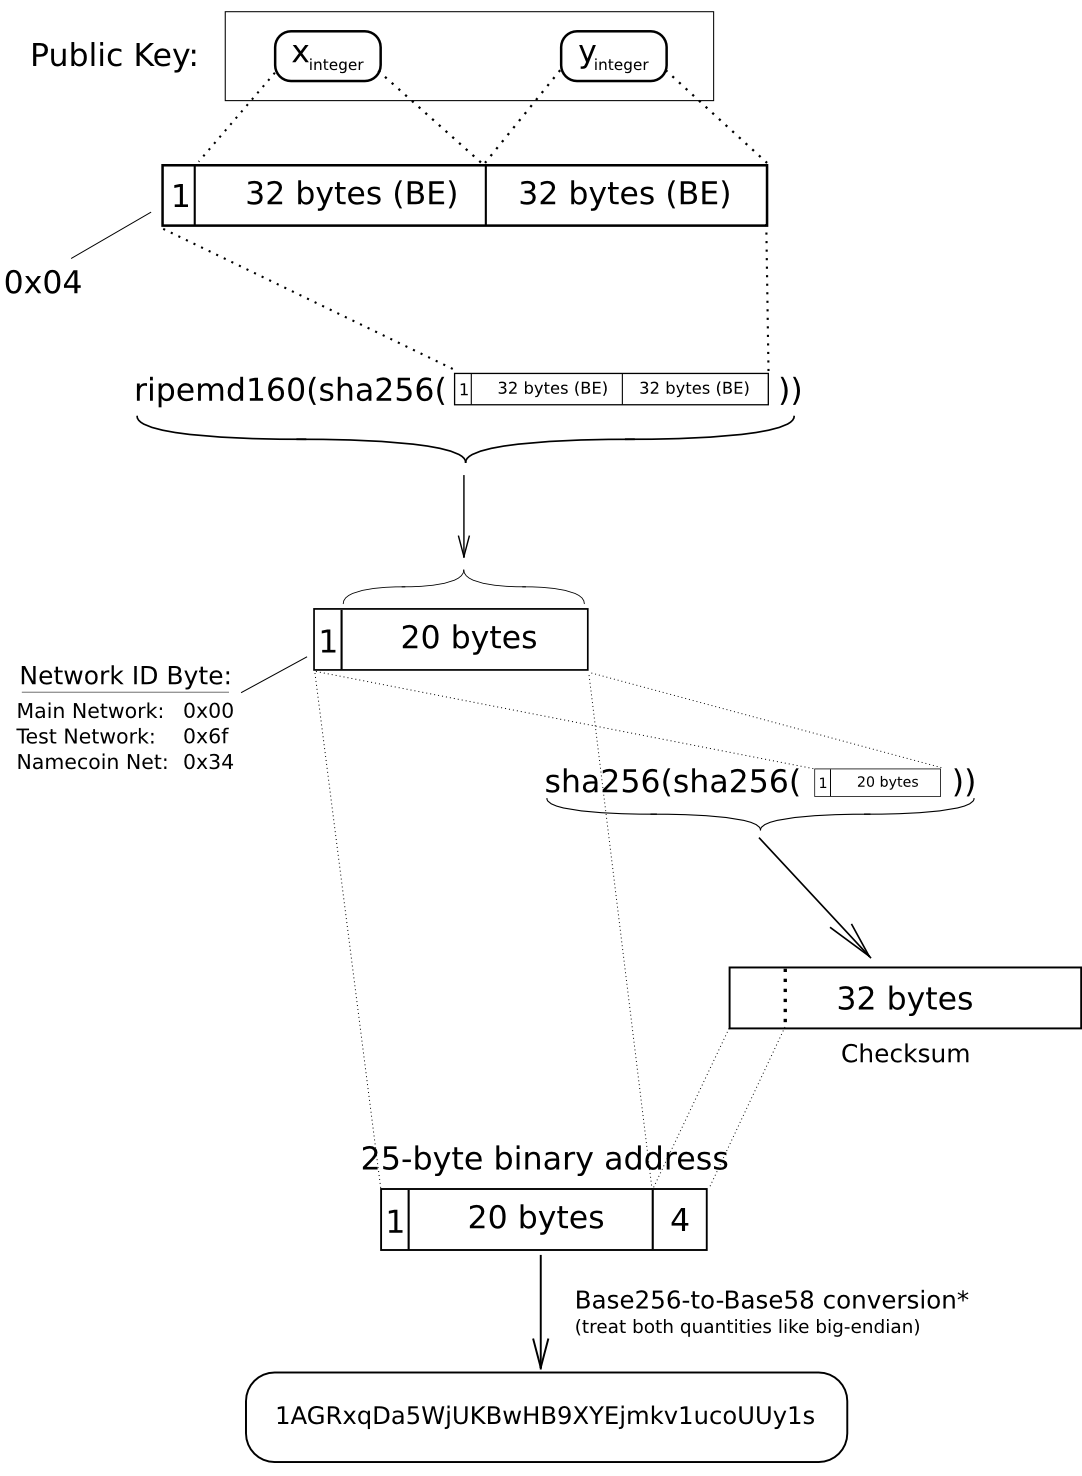
\includegraphics{img/capuno/PubKeyToAddr.png}
	\caption{Creazione di un indirizzo Bitcoin a partire dalla chiave pubblica~\emph{\cite{bitaddress2020}}.}
	\label{fig:bit_address}
\end{figure}

Quando un nodo crea una transazione, presenta la sua chiave pubblica e firma la transazione per dimostrare di essere il proprietario di quel conto. In questo modo, chiunque nella rete, con queste due informazioni, può verificare che il nodo è realmente il proprietario di una certa quantità di bitcoin spesi in una transazione. \'E chiaro che chiunque in possesso della chiave privata di un nodo, può spendere a suo piacimento i bitcoin associati al relativo bitcoin address. Per questo, e anche per anonimizzare i creatori delle transazioni, un wallet genera ad ogni transazione una nuova coppia di chiavi.

Un wallet, come si già è detto in precedenza, è un client che memorizza le chiavi digitali di un nodo. Può essere: (1) \emph{non-deterministico} e generare chiavi private in modo totalmente randomico, per cui il wallet è un database che memorizza queste chiavi private, e (2) \emph{deterministico} e generare delle chiavi private a partire da un \emph{seed}, che può essere anche una password digitata da un utente, per cui non ha bisogno di memorizzare alcuna chiave.


\subsection{Transazioni}

Le transazioni ricoprono un ruolo fondamentale in Bitcoin e nelle tecnologie di blockchain in generale. Le transazioni sono delle strutture dati che codificano un trasferimento di bitcoin da una o più sorgenti, denominate \emph{input}, ad una o più destinazioni, denominate \emph{output}. I campi di una transazione sono riportati nella Tabella~\ref{tab:tx_fields}.

\begin{table}
	\centering
	\begin{tabular}{lll}
		\toprule
		Dimensione&Campo&Descrizione\\
		\midrule
		4 byte&Versione&Specifica la versione del protocollo\\
		1-9 byte&Contatore input&Indica quanti input sono inclusi\\
		variabile&Input&Lista di uno o più input\\
		1-9 byte&Contatore output&Indica quanti output sono inclusi\\
		variabile&Output&Lista di uno o più output\\
		4 byte&Time&Timestamp Unix\\
		\bottomrule
	\end{tabular}
	\caption{I campi di una transazione.}
	\label{tab:tx_fields}
\end{table}

Vediamo ora il ciclo di vita di una transazione. Ogni nodo nella rete può generare una transazione. La transazione contiene una firma che dimostra che il nodo possiede i bitcoin specificati nell'input. Essa viene quindi inviata in broadcast, raggiungendo tutti i nodi della rete. Questa viene messa nella lista delle transazioni in attesa, o \emph{pending transaction}, verificata da ogni nodo, e se valida, ovvero conforme alle regole di consenso, è inclusa all'interno di un blocco insieme ad altre transazioni. Se sul blocco viene risolto un puzzle crittografico, esso viene aggiunto in coda alla blockchain. Una transazione può essere creata da un nodo anche se questo è offline. Una volta tornato online può inviare la nuova transazione al resto della rete.

Non esiste il concetto di conto relativo ad un account Bitcoin, per cui le transazioni formalmente non spostano valuta da un conto all'altro. In altre parole non esiste un database che memorizza i conti degli utenti, come in altre tecnologie blockchain presentate nei prossimi paragrafi, ma i bitcoin posseduti da un certo indirizzo sono calcolati scandendo tutta la blockchain dal blocco iniziale al blocco attuale, considerando le \emph{unspent transactions output}, o \textit{UTXO}. Le UTXO sono i mattoncini con cui vengono generate le transazioni. Ad ogni UTXO è associato un valore espresso in \emph{satoshi}, dove 1 satoshi è equivalente a $10^{-8}$ bitcoin, e sono bloccate da un segreto di cui è a conoscenza solo il possessore. I satoshi corrispondono ai centesimi presenti nelle valute tradizionali, come l'Euro o il Dollaro, solo che, a differenza di queste ultime in cui l'unità di base può essere suddivisa in massimo 100 parti, il bitcoin, può essere suddiviso fino a 100 milioni di parti.

Le UTXO corrispondono agli output di una transazione, facente parte di un blocco della blockchain, che non è stata ancora spesa da un'altra transazione. Gli output di una transazione consistono in due parti:

\begin{enumerate}
	\item il valore espresso in satoshi da trasferire;
	\item un \emph{locking script}, che specifica il modo in cui i bitcoin possono essere sbloccati.
\end{enumerate}

Per semplicità un locking script può essere pensato come l'indirizzo della destinazione, che diventerà, una volta che la transazione è stata accettata e quindi aggiunta in blockchain, il proprietario della quantità di bitcoin indicati nella transazione stessa.

Ogni input in una transazione è un rifermento ad una UTXO. In particolare si indica l'UTXO da utilizzare come sorgente specificando l'hash della transazione e l'indice dell'output nella transazione considerata. Il creatore della transazione deve includere un \emph{unlocking script} per ogni UTXO, contenente una firma che dimostri che il peer che ha creato la transazione è proprietario di quei bitcoin.

Molte transazioni includono delle \emph{tasse}. Esse hanno un triplice scopo. Il primo è incentivare i miner a scegliere la propria transazione. I miner, oltre a ricevere un compenso per la creazione del blocco, ricevono le tasse di tutte le transazioni presenti nel blocco creato. Infatti, quando i miner provano a generare un blocco, scelgono dal proprio pool di transazioni in attesa quelle con le tasse più alte. Il secondo è quello di incentivare un peer ad essere un miner, in modo tale che la rete sia più sicura. Come si vedrà successivamente, la sicurezza dell'intero sistema aumenta con l'aumentare dei nodi che partecipano alla rete. L'ultimo, disincentiva nodi malevoli a \emph{spam} di transazioni, perché questi si troverebbero a spendere una piccola quota in tasse per ogni transazione generata. La quantità di tasse da pagare per una transazione normalmente dipende dalla sua dimensione in byte, in genere sui 370 byte, ma dipende anche dalle richieste di mercato. Al momento di scrittura di questa tesi, per una transazione di circa 370 byte composta da 2 input e 2 output, affinché sia accettata entro 2 blocchi, quindi entro 20 minuti, sono necessari 34k satoshi, pari a 3.20 USD (fonte~\cite{bitcoin_fee_calculator}).

Come si è visto, nella struttura dati di una transazione non è presente un campo tasse esplicito. Le tasse sono infatti implicite e sono calcolate da ogni miner come la differenza tra la somma degli input e la somma degli output. In formule,
\begin{equation*}
	Tasse = \sum T_{in} - \sum T_{out}
\end{equation*}
dove $T_{in}$ e $T_{out}$ indicano l'input e l'output di una transazione $T$, rispettivamente.

Gli script sono il sistema con cui i peer Bitcoin validano le transazioni. Come si è detto in precedenza, ad ogni UTXO è associato un locking script, che rappresenta le condizioni che un nodo deve soddisfare per poter utilizzare i bitcoin contenuti in essa. L'input di una transazione, riferito ad uno specifico UTXO, deve fornire un unlocking script, che contiene solitamente una firma che sblocca i fondi. Durante la validazione di una transazione, il peer esegue prima l'unlocking script e usa il suo output come input per il locking script. Se non ci sono errori e le condizioni nel locking script sono soddisfatte, ovvero l'intera operazione restituisce \emph{true}, allora la transazione è considerata valida.
Gli script sono scritti in un linguaggio stack-based, in cui sono presenti istruzioni aritmetico-logiche, istruzioni per il calcolo di hash, di verifiche di chiavi pubbliche, istruzione condizionale, ma non loop, il che lo rende \emph{Turing incompleto}. Questo fa si che non è possibile creare un loop infinito e causare quindi un \emph{Denial-of-Service}. Grazie ad un linguaggio di scripting è possibile scrivere un'infinità di script che danno modo di esprimere qualsiasi condizione. La più usata è certamente la \emph{Pay to public key hash}, nota anche con P2PKH, che consente di specificare l'indirizzo Bitcoin a cui trasferire una certa somma di bitcoin. La Figura~\ref{fig:p2pkh} mostra un esempio di locking e unlocking script per una transazione P2PKH. \'E possibile creare anche fondi sbloccabili solo da più utenti insieme o anche da una certa data in poi. Questi sono solo alcuni degli esempi che è possibile creare.

\begin{figure}
	\centering
	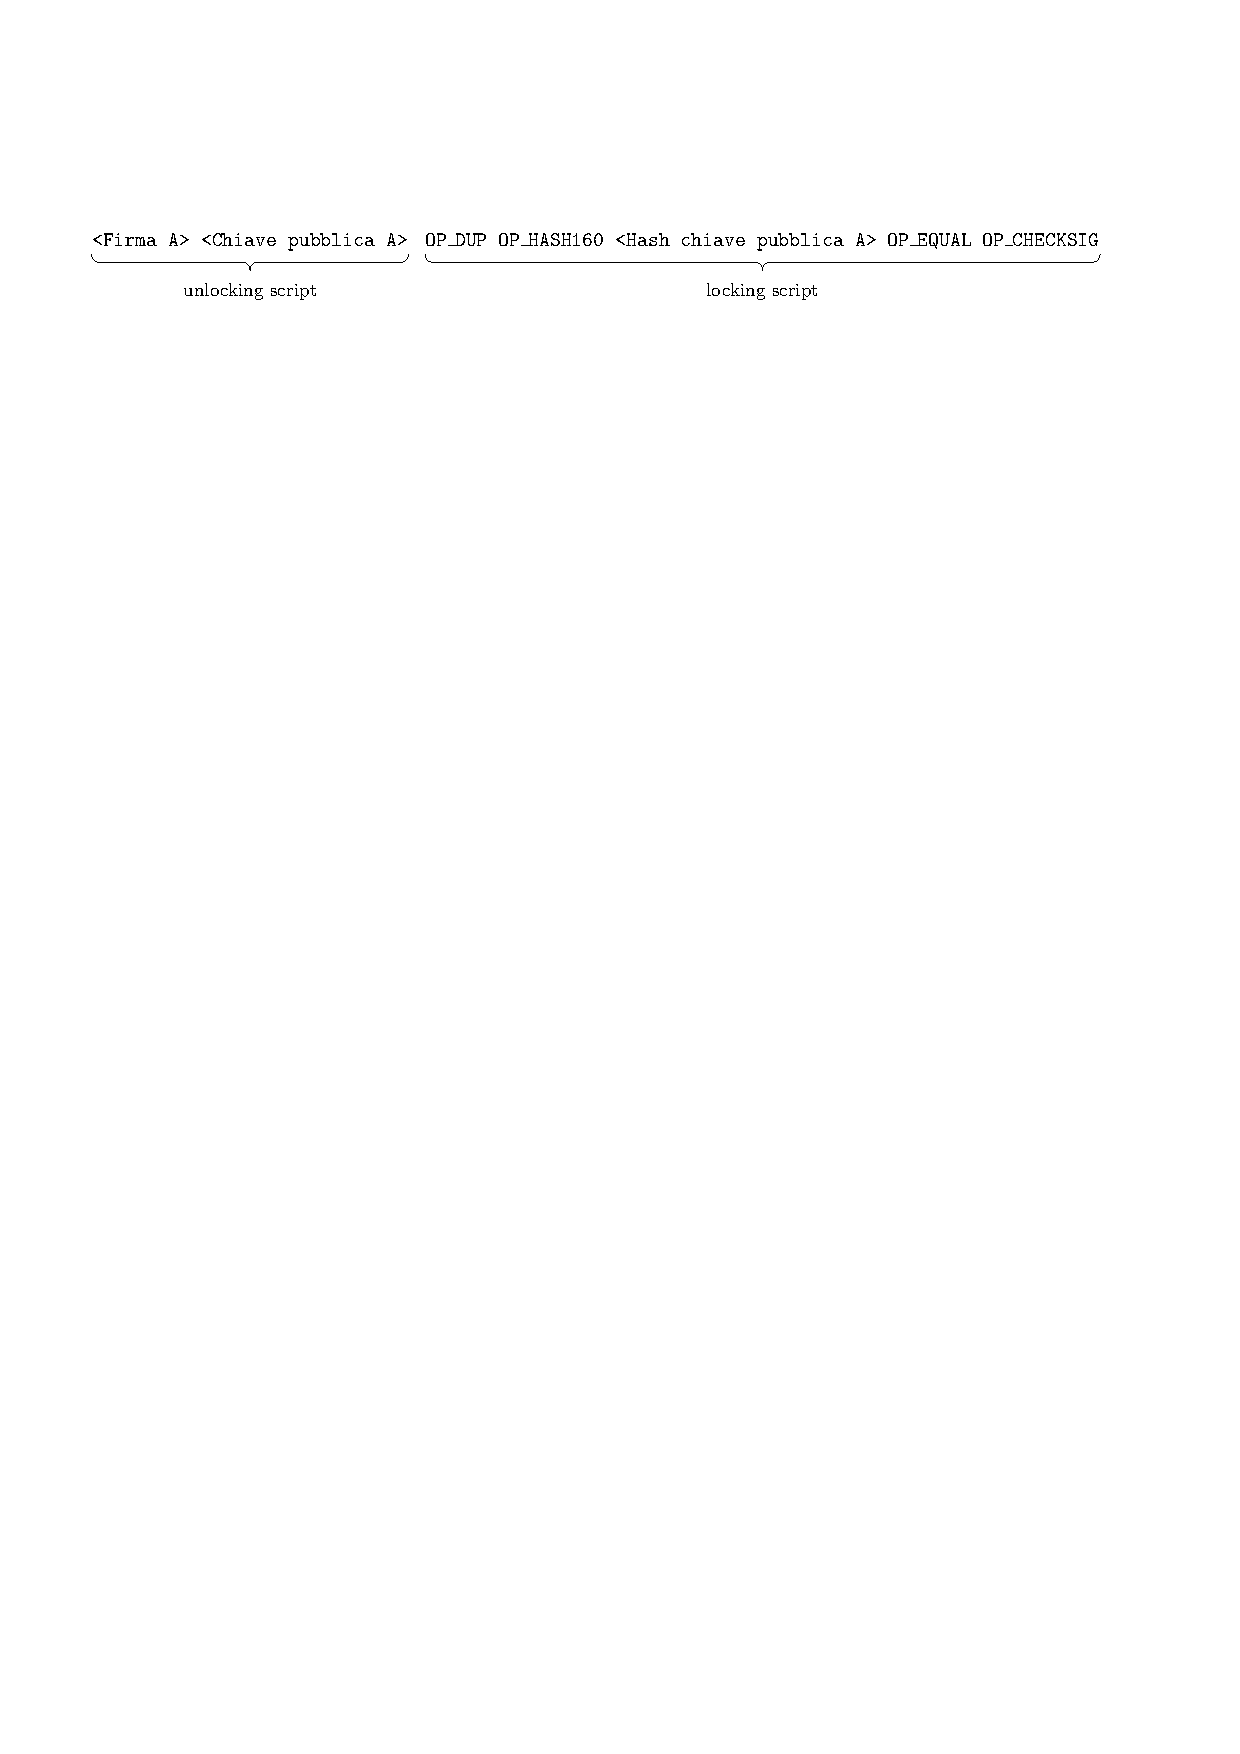
\includegraphics[scale=0.78]{img/capuno/p2pkh.pdf}
	\caption{Esempio di locking ed unlocking script per una transazione P2PKH. La transazione è generata dall'utente $A$ che deve dimostrare nell'unlocking script la propria identità.}
	\label{fig:p2pkh}
\end{figure}


\subsection{Mining}
Il mining ha lo scopo principale di confermare le transazioni in attesa, generando un nuovo blocco da aggiungere alla blockchain, con un meccanismo completamente decentralizzato, dove ogni nodo della rete, o \emph{miner}, può contribuire al processo. Non è necessario nessun comitato speciale o un'autorità centrale che gestisca tutta l'operazione. Circa ogni 10 minuti viene creato un nuovo blocco contenente le transazioni confermate da aggiungere in coda alla blockchain.
Il mining ha anche lo scopo di generare nuovi bitcoin, da qui il termine mining, che allude all'estrazione di pietre prezione dalle miniere, con una decrescita esponenziale nel tempo di creazione di valuta. Ogni nodo che riesce ad inserire un nuovo blocco alla blockchain, viene ricompensato con una quantità fissa di bitcoin, dimezzata ogni 210.000 blocchi (circa ogni 4 anni), partendo da 50 bitcoin da gennaio 2009. Dall'11 maggio 2020, infatti, la ricompensa per i miner è di $6.25$ bitcoin. Quindi, la ricompensa decresce esponenzialmente fino al 2140, quando circa 21 milioni di bitcoin (per l'esattezza 2.099.999.997.690.000 satoshi) saranno generati, approssimativamente dopo 13.44 milioni di blocchi. Un miner riceve come ricompensa anche le tasse delle transazioni che ha inserito nel nuovo blocco. Per cui dopo il 2140, i miner riceveranno come ricompensa solo le tasse presenti nelle transazioni. Quello della ricompensa è ovviamente un meccanismo atto ad incentivare la presenza di più miner, che concorrono alla conferma di nuove transazioni, aumentando in questo modo la sicurezza dell'intera rete.

Finora si è parlato dei miner che cercano di creare un nuovo blocco da aggiungere alla blockchain, senza specificare il come. Vediamo quindi come i miner creano i nuovi blocchi della blockchain, secondo un meccanismo di consenso decentralizzato, che rappresenta il vero contributo di Satoshi Nakamoto alle reti P2P, secondo cui tutti i nodi presenti nella rete concordano su un certo stato della blockchain, senza un'autorità centrale che governi tutto. Il consenso è infatti raggiunto in maniera asincrona su tutta la rete, ed ogni nodo può vedere lo stesso stato della blockchain.
Quando una transazione viene generata da un qualsiasi peer della rete, essa viene inviata in broadcast a tutti i nodi della rete. Ogni nodo che riceve una transazione, prima di inviarla ai peer successivi, effettua numerosi controlli di validità, come la conformità alle regole sintattiche e regole di consenso, come (1) verificare che la transazione non faccia \emph{double spending}, ovvero si utilizza più di una volta la stessa UTXO, confrontando gli input della transazione con gli output delle transazioni nei blocchi della blockchain e con quelle del pool delle transazioni, (2) verificare che la somma degli input sia maggiore della somma degli output, e (3) verificare che l'output dell'unlocking script di ogni input sblocchi il locking script dell'UTXO a cui l'input si riferisce. Se una transazione soddisfa tutti questi requisiti, viene inserita nel pool delle transazioni del peer, uno spazio di memoria temporaneo in cui risiedono le transazioni valide in attesa di essere inserite in un blocco, per poi essere inviata in broadcast ad ogni peer vicino. Ogni peer effettua tutti questi controlli. A questo punto, ogni miner sceglie le transazioni che formeranno il prossimo blocco, denominato \emph{candidate block}, dal pool delle transazioni. I primi 50 kilobyte di un blocco sono formati da quelle transazioni ad \emph{alta priorità}: la priorità viene calcolata in base all'età dell'UTXO che dovrà essere spesa, ovvero in base alla profondità a cui si trova nella blockchain la transazione contenente l'UTXO rispetto al blocco corrente. La formula per il calcolo della priorità è la seguente:

\begin{equation*}
	Priority = \frac{\sum_i  value(T_i) * age(T_i)}{size(T)}
\end{equation*}

dove $value(T_i)$ è il valore dell'input $i$ della transazione $T$ espresso in satoshi, $age(T_i)$ è la profondità dell'UTXO a cui si riferisce l'input $i$ della transazione nella blockchain, e $size(T)$ è la dimensione della transazione espressa in byte.
Questo consente alle transazioni di essere inserite anche se non hanno alcuna tassa.
Il resto del blocco, che ha una dimensione massima di 4 megabyte, viene riempito dalle transazioni presenti nel pool che hanno una tassa maggiore. Questo perché tutte le tasse presenti nelle transazioni vengono ricevute dal nodo miner che ha creato il blocco.
Infine, la prima transazione che viene inserita nel blocco è quella denominata \emph{coinbase}, una transazione speciale che non contiene alcun input, il cui output contiene come valore la somma delle tasse presenti nelle altre transazioni del blocco e la ricompensa per il blocco creato e avete come indirizzo destinazione quello del nodo miner. La coinbase rappresenta la ricompensa al miner per il lavoro svolto.

Vediamo ora come funziona l'algoritmo di consenso. Una volta costruito il blocco, esso deve essere \emph{minato}, ovvero si deve trovare la soluzione all'algoritmo \emph{Proof-of-Work} che rende valido il blocco. Esso si basa sugli \emph{hash crittografici}, denominati in seguito più semplicemente con hash. Un hash è una funzione che dato un input di una qualsiasi dimensione, produce una stringa di output di dimensioni fisse. Essa è semplice da calcolare, ma difficile da un punto di vista computazionale invertire, ovvero dato un hash $h$, calcolare l'input $S$ tale che $h = hash(S)$. Ad esempio, la funzione SHA256, utilizzata in Bitcoin, produce un output di 256 bit. Inoltre, un'altra proprietà fondamentale è che a fronte dello stesso input si produce lo stesso output, perciò l'hash è una funzione deterministica. Secondo Proof-of-Work un miner deve trovare un blocco, tale che l'hash del suo header sia minore di una certa soglia, denominata \emph{target}. Questo viene svolto variando una parte dell'header del blocco denominato \emph{nounce}, e viene inserito nell'header del blocco come prova del lavoro svolto. Poiché gli hash non seguono un certo pattern, l'unico modo di trovare un nounce che faccia assumere all'header del blocco un valore minore del target è quello di tentare tutte le combinazioni. Essendo l'hash facile da calcolare, verificare il lavoro svolto da un miner è un compito semplice. Il primo nodo miner che riesce a trovare una soluzione a questo puzzle crittografico, è il vincitore di questa competizione ed invia in broadcast il blocco minato come prova del lavoro svolto. Proof-of-Work, in altre parole, consente di eleggere un leader randomicamente con una probabilità dipendente dalla sua potenza computazionale in rapporto a quella della rete (denominata \emph{hash power}), che propone il nuovo blocco da inserire in blockchain.
Il target determina la difficoltà nel trovare un blocco che soddisfi le condizioni di consenso, in quanto questo determina un aumento esponenziale del numero di tentativi da svolgere per risolvere il problema. Poichè la potenza computazionale aumenta nel tempo, e quindi il numero di hash calcolabili nell'unità di tempo, c'è un meccanismo che reimposta il target ogni 2016 blocchi, circa ogni 2 settimane, in modo tale che in media un blocco sia minato in 10 minuti. Il miner che mina il blocco $k$ tale che $k$ sia divisibile per 2016, determina il nuovo target sulla base del tempo impiegato a trovare gli ultimi 2016 blocchi: se il tempo è maggiore di 20160 minuti aumenta il target, diminuendo quindi la complessità, se è minore diminuisce il target, aumentando la complessità del problema.
Quando gli altri miner ricevono il blocco minato da un altro miner, cessano di minare il proprio blocco ed iniziano a lavorare sul successivo, utilizzando lo stesso approccio appena descritto.

Può capitare che due miner nella rete riescano a minare quasi contemporaneamente un blocco, per cui i vicini potrebbero lavorare a loro volta su viste della blockchain differenti. Questo genera nella blockchain delle \emph{fork}. In questo caso alcuni nodi della rete possiedono una vista differente della blockchain. Il problema viene risolto da ogni nodo scegliendo il ramo più lungo, in modo da convergere allo stesso stato della blockchain. Il processo è denominato \emph{fork resolution}. A causa della possibilità di fork, una transazione è considerata confermata quando raggiunge una profondità maggiore di sei blocchi (quindi, in media dopo un'ora).


\subsection{Attacchi noti}\label{attacks}

\paragraph{51\% attack}
Qualsiasi tecnologia di blockchain per sua natura si basa su un meccanismo di consenso distribuito che garantisce una mutua fiducia. Se nelle blockchain basate su Proof-of-Work un miner possiede più del 50\% dell'hash power, può mettere in atto l'\textit{attacco 51}\% (o \emph{attacco Sybil}~\cite{douceur2002sybil}). Questo gli consente di ottenere il 100\% delle ricompense dal mining, poichè riuscirebbe a creare catene di blocchi sicuramente più lunghe di qualsiasi altro miner. Inoltre può fare un \emph{double spending}, in cui si utilizza la stessa UTXO come input alle transazioni, eliminare dalla blockchain gli ultimi blocchi confermati ed eventualmente corrompere la blockchain stessa.
In una tecnologia come Bitcoin che incentiva economicamente i nodi a diventare miner e che ha raggiunto nel tempo un numero di nodi elevato, e quindi un grande hash power, un simile attacco è molto improbabile. Sicuramente non sono escluse da questo attacco le blockchain di piccole dimensioni, che hanno un hash power di gran lunga minore di quello di Bitcoin: esempi di cripto-valute che sono state vittime del 51\% attack sono Monacoin~\cite{monacoin2018attack}, Bitcoin Gold~\cite{bitcoingold2020attack} e ZenCash~\cite{zencash2020attack}.
In realtà l'avvento delle mining pool in Bitcoin, in cui più miner mettono a disposizione la propria potenza computazionale al servizio di un gruppo di più miner che divide il compenso in modo proporzionale all'hash power condiviso, apre la possibilità ad un'organizzazione del genere ad un 51\% attack se la somma totale dell'hash power di tutti i nodi iscritti supera il 50\% dell'intero hash power della rete.

\paragraph{Eclipse attack}
L'\emph{eclipse attack} è un attacco perpetrato ai danni di una singola vittima. Un attaccante, che controlla un gran numero di nodi, ad esempio una botnet, può isolare un nodo dal resto della blockchain. Questo gli consente di mostrare una blockchain differente da quella che è in realtà e di sfruttare la potenza computazionale della vittima per i suoi comportamenti malevoli. La Figura~\ref{fig:eclipse_attack} mostra una rappresentazione di un attacco Eclipse. Heilman et al.~\cite{heilman2015eclipse}, mostrano che è possibile utilizzare un attacco eclipse come base per altri attacchi.

\begin{figure}
	\centering
	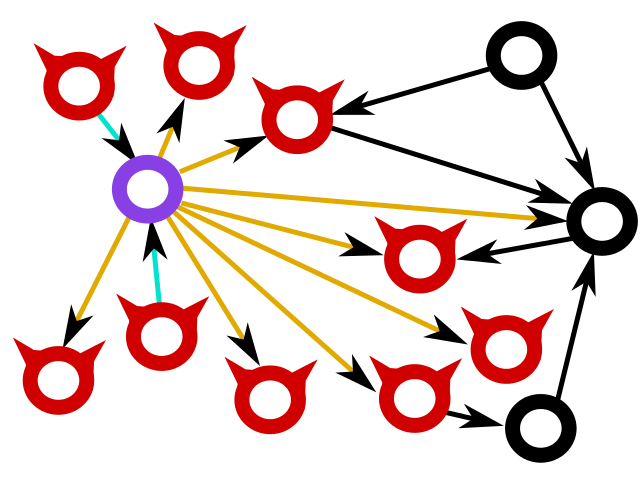
\includegraphics[scale=0.3]{img/capuno/eclipse_attack.png}
	\caption{Rappresentazione di un attacco eclipse in cui un nodo è isolato dal resto della rete. \emph{Fonte~\cite{heilman2015eclipse}}}
	\label{fig:eclipse_attack}
\end{figure}

\begin{itemize}
	\item \textbf{Engineering block races}: Quando due miner riescono a minare un blocco nello stesso momento, solo uno entra a far parte della blockchain, mentre l'altro diventa un blocco \emph{orfano} ed il miner che ha minato questo blocco non riceve alcuna ricompensa. Un attaccante che eclissa più di un miner, accumula i blocchi minati dai miner attaccati, per poi rilasciarli alla rete solo quando un miner non attaccato scopre un blocco. In questo modo i blocchi minati dalle vittime diventano orfani. Questo porta quindi ad uno spreco delle risorse degli attaccati.
	\item \textbf{Splitting mining power}: Si eclissa un certo numero di miner in modo da ridurre l'hash power della rete e consentire più facilmente un 51\% attack.
	\item \textbf{Selfish mining}: Questo attacco consente ad un attaccante di sprecare risorse a miner vittime o di ottenere una ricompensa maggiore. L'attaccante mantiene private una lista di blocchi che ha minato ed elimina i blocchi minati dai miner eclissati che competono con i blocchi che lui ha minato. Nello stesso tempo sfrutta la potenza computazionale dei nodi vittime tentando di creare un fork più grande rispetto alla catena di blocchi della vera blockchain.
	\item \textbf{0-confirmation double spend}: Si ha nel caso di \emph{0-confirmation transaction}, dove un venditore spedisce, nel caso di vendita online, o rilascia, nel caso di vendita in un negozio fisico, un bene ad un cliente prima che questa sia confermata in un blocco. Questo accade quando non si vogliono attendere i circa 10 minuti di conferma di una transazione. L'attaccante effettua un eclipse attack al venditore, inviandogli una transazione $T$ per comprare i beni ed una transazione $T'$ al resto della rete, facendo un \emph{double spending}. Il mercante rilascia il prodotto al cliente malevolo e poiché è eclissato non può inviare $T$ al resto della rete. Quindi l'attaccante ottiene un prodotto senza aver pagato.
	\item \textbf{N-confirmation double spend}: In questo caso, a differenza del precedente, un mercante rilascia un bene al suo cliente solo se la transazione si trova almeno a profondità $N-1$ nella blockchain. L'attaccante invia la transazione ai nodi eclissati, che la inglobano in una vista \emph{vecchia} della blockchain, tra cui è presente anche il commerciante. L'attaccante, dopo aver ricevuto il prodotto, mostra alle vittime eclissate la vera blockchain, aggiornata nel frattempo dai nodi non eclissati. La blockchain vista dai nodi eclissati diventa orfana, poiché è un fork più corto rispetto alla vista della blockchain del resto della rete. La transazione creata dall'attaccante viene quindi eliminata. Anche in questo caso, l'attaccante ottiene un prodotto senza aver pagato.
\end{itemize}


\section{Blockchain Scalability Trilemma}
Sebbene il \emph{blockchain scalability trilemma}~\cite{trilemma1} influisca sull'analisi e progettazione di tecnologie di blockchain, non è presente una definizione formale in letteratura, anche se è citato in numerosi lavori, come~\cite{xie2019survey, zhou2020solutions}. Il termine~\cite{sharding2020site} fu coniato da Vitalik Buterin, creatore di \emph{Etherium}, una blockchain basata su Proof-of-Work, individuando le tre caratteristiche che una blockchain deve possedere per allargare i propri confini a livello globale: \emph{decentralizzazione}, \emph{sicurezza} e \emph{scalabilità}. Il \emph{trilemma} afferma che una blockchain può possederne solo due sulle tre disponibili. Il blockchain scalability trilemma si può rappresentare con un triangolo, come in Figura~\ref{fig:trilemma}, ai cui vertici ci sono le tre proprietà e in cui l'ottimo è al centro.

\begin{figure}
	\centering
	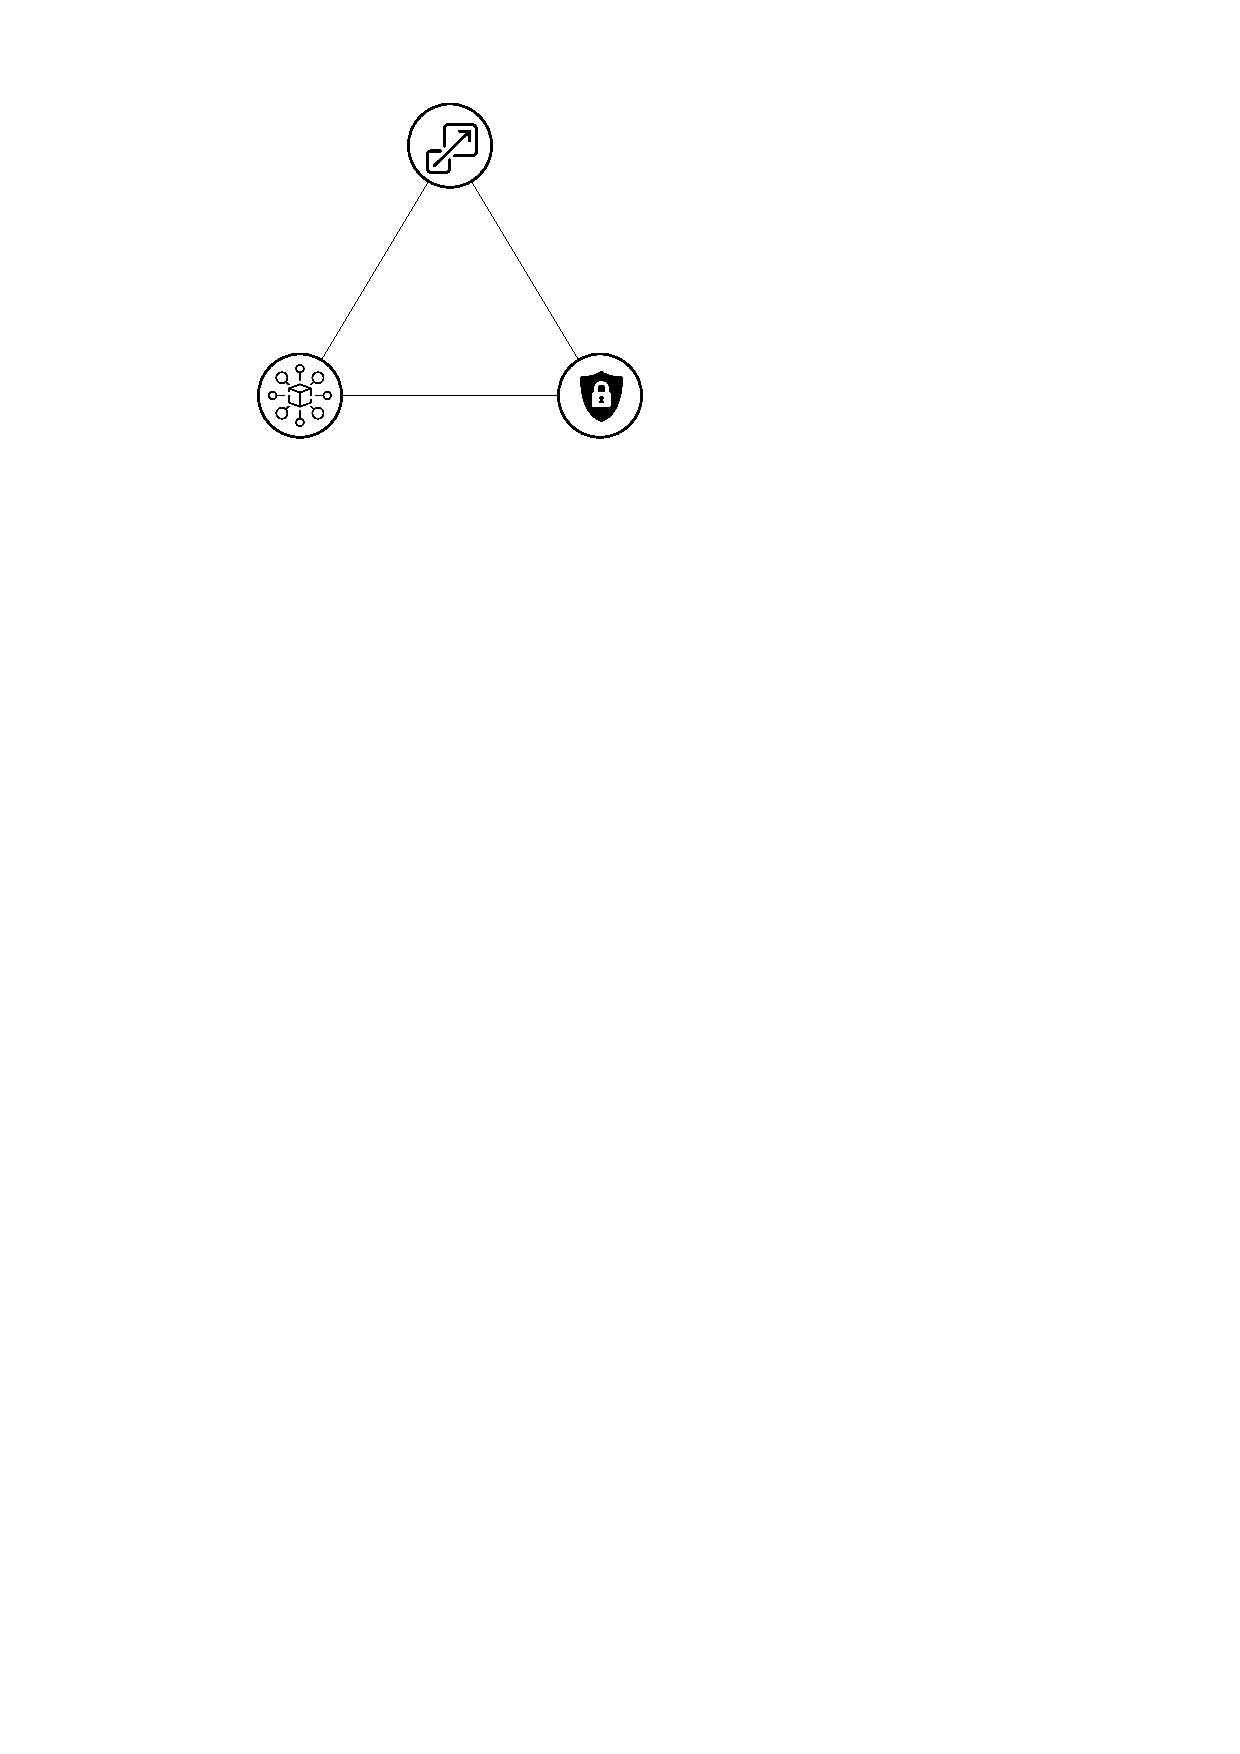
\includegraphics{img/capuno/trilemma.pdf}
	\caption{Rappresentazione del blockchain scalability trilemma. Secondo il trilemma una blockchain può trovarsi su uno dei lati del triangolo e non nel centro, rappresentante l'ottimo.}
	\label{fig:trilemma}
\end{figure}

Vediamo in dettaglio i tre elementi fondamentali del trilemma.

\paragraph{Decentralizzazione}
Per decentralizzazione si intende il fatto che le transazioni sono validate e confermate da un gruppo di nodi e non da un'autorità centrale o un comitato speciale, come accade in sistemi tradizionali, per cui le decisioni sono ottenute da un consenso distribuito. Quindi non è necessario riporre fiducia su una terza parte durante una qualsiasi operazione. In altre parole, le decisioni sono ottenute democraticamente da tutti i partecipanti alla rete, ed ogni proposta di cambiamento nel protocollo può essere accettata se più del 50\% dei partecipanti è favorevole. Un esempio è Bitcoin Cash, un fork di Bitcoin avvenuto il 1 agosto 2017~\cite{bcash}, in cui si portò ad 8 MB la dimensione massima di un blocco, in modo da consentire un numero maggiore di transazioni accettate.
\'E chiaro che la decentralizzazione ha come conseguenza una \emph{qualità} di decisione più alta rispetto ad una presa da un'autorità centrale, poiché la conferma è ottenuta da più nodi. Il trade-off è però la velocità di conferma: se una transazioni richiede una conferma da più partecipanti la velocità è minore di una decisione presa da un'autorità centrale.

\paragraph{Scalabilità}
La scalabilità è la proprietà che consente realmente un'adozione a livello globale. Essa si riferisce al fatto che un sistema possa adattarsi ad un incremento di carico. Ad esempio, le due tecnologie di blockchain ad oggi più utilizzate, Bitcoin e Ethereum, posso gestire un carico massimo di 7 e 12 TPS\footnote{TPS = transazioni al secondo}
al contrario di Visa, che può raggiungere le 65.000 TPS~\cite{visatps}. EOS~\cite{xu2018eos}, una blockchain progettata per essere scalabile, ha un throughput dichiarato di circa 2000 TPS, ma promette di poter processare milioni di transazioni in futuro, tuttavia ad un prezzo: la decentralizzazione.

\paragraph{Sicurezza}
La sicurezza deve essere il requisito fondamentale in una blockchain. Se la sicurezza è povera o del tutto assente, un attaccante può spendere più volte la stessa quantità di denaro (\emph{double spending}), arricchendo se stesso a scapito di altri ed arrivare a modificare lo stato della blockchain, che per sua natura è immutabile. Questo può succedere ad esempio nel 51\% attack, presentato nel Paragrafo~\ref{attacks}.

\paragraph*{}
\'E importante notare che il blockchain scalability trilemma non è un teorema, come lo è il \textit{CAP theorem}, un teorema fondamentale nell'ambito dei sistemi distribuiti. Esso sottolinea la difficoltà nel creare un sistema decentralizzato, sicuro e scalabile. Le blockchain sono ancora tecnologie giovani, poco mature per cui c'è ancora tanta strada da fare, in grado di migliorare ciò che già è stato fatto. Bitcoin, ad esempio, è una blockchain altamente sicura e decentralizzata, ma non scalabile: il numero di transazioni massime supportate è infatti di 7 TPS. Sebbene, non sarà utilizzabile a livello globale come unica valuta, rappresenta nella storia dell'informatica un punto di svolta, dimostrando che una cripto-valuta digitale in un sistema P2P, in cui non è necessario riporre la fiducia su un'autorità centrale o si è soggetti a regole imposte dalla medesima, è possibile e attuabile in pratica.


\section{Strutture dati autenticate}\label{sec:ads}

Come si è visto nella Paragrafo~\ref{sec:blockchain}, ogni block header della blockchain contiene un riassunto di tutte le transazioni presenti nel blocco, denominato \emph{root-hash}, ed ottenuto da un \textit{Merkle Tree} (\textit{MHT}). Esso fa parte della famiglia delle \emph{strutture dati autenticate}.

Una struttura dati autenticata (ADS) è una struttura dati che permette una verifica di integrità dei dati memorizzati. Permettono ad un client di verificare l'autenticità e l'integrità di una risposta ottenuta da un server non fidato mediante una prova, denominata \emph{proof}. In altre parole, le operazioni effettuate da una parte esterna non fidata, denominato \emph{prover}, possono essere verificate efficientemente da un client, il \emph{verifier}.

Supponiamo di trovarci nel seguente scenario. Un client ha bisogno di memorizzare una certa quantità di dati che eccede le sue disponibilità di memorizzazione fisica. Può memorizzare i suoi dati su un server esterno che ha una grande capacità di memorizzazione, come ad esempio un servizio di cloud storage. Il client vuole essere sicuro che la versione dei file che memorizza in cloud sia l'ultima e che nessuno possa modificare il contenuto dei suoi file. Questo problema può essere risolto mediante le strutture dati autenticate, senza che il client memorizzi l'intera struttura dati e senza memorizzare l'hash di ogni singolo file. In quest'ultimo caso infatti dovrebbe memorizzare un numero di hash lineare con il numero di file che ha memorizzato in cloud. Applicazioni del genere sono molto frequenti, anche nel caso di Bitcoin, in cui esistono client \emph{leggeri}, i cosiddetti \emph{thin client}, che memorizzano solo l'header dei blocchi della blockchain, mentre tutte le transazioni contenute nei blocchi sono memorizzati su un server esterno. Una realizzazione di un protocollo efficiente che fa uso di ADS si può trovare in \cite{pennino2019pipeline} e \cite{gdm}.

Un'implementazione efficiente di un'ADS è il Merkle Tree, utilizzato per la realizzazione di dizionari autenticati. Dato un insieme di elementi $V$, il Merkle Tree $T$ è un albero binario completo bilanciato avente come foglie gli hash degli elementi in $V$, mentre i nodi intermedi sono il risultato dell'hash della concatenazione dei nodi figli. Il root di $T$ contiene il \emph{root-hash} di $T$. La Figura~\ref{fig:mht} mostra un esempio di Merkle Tree.

\begin{figure}
	\centering
	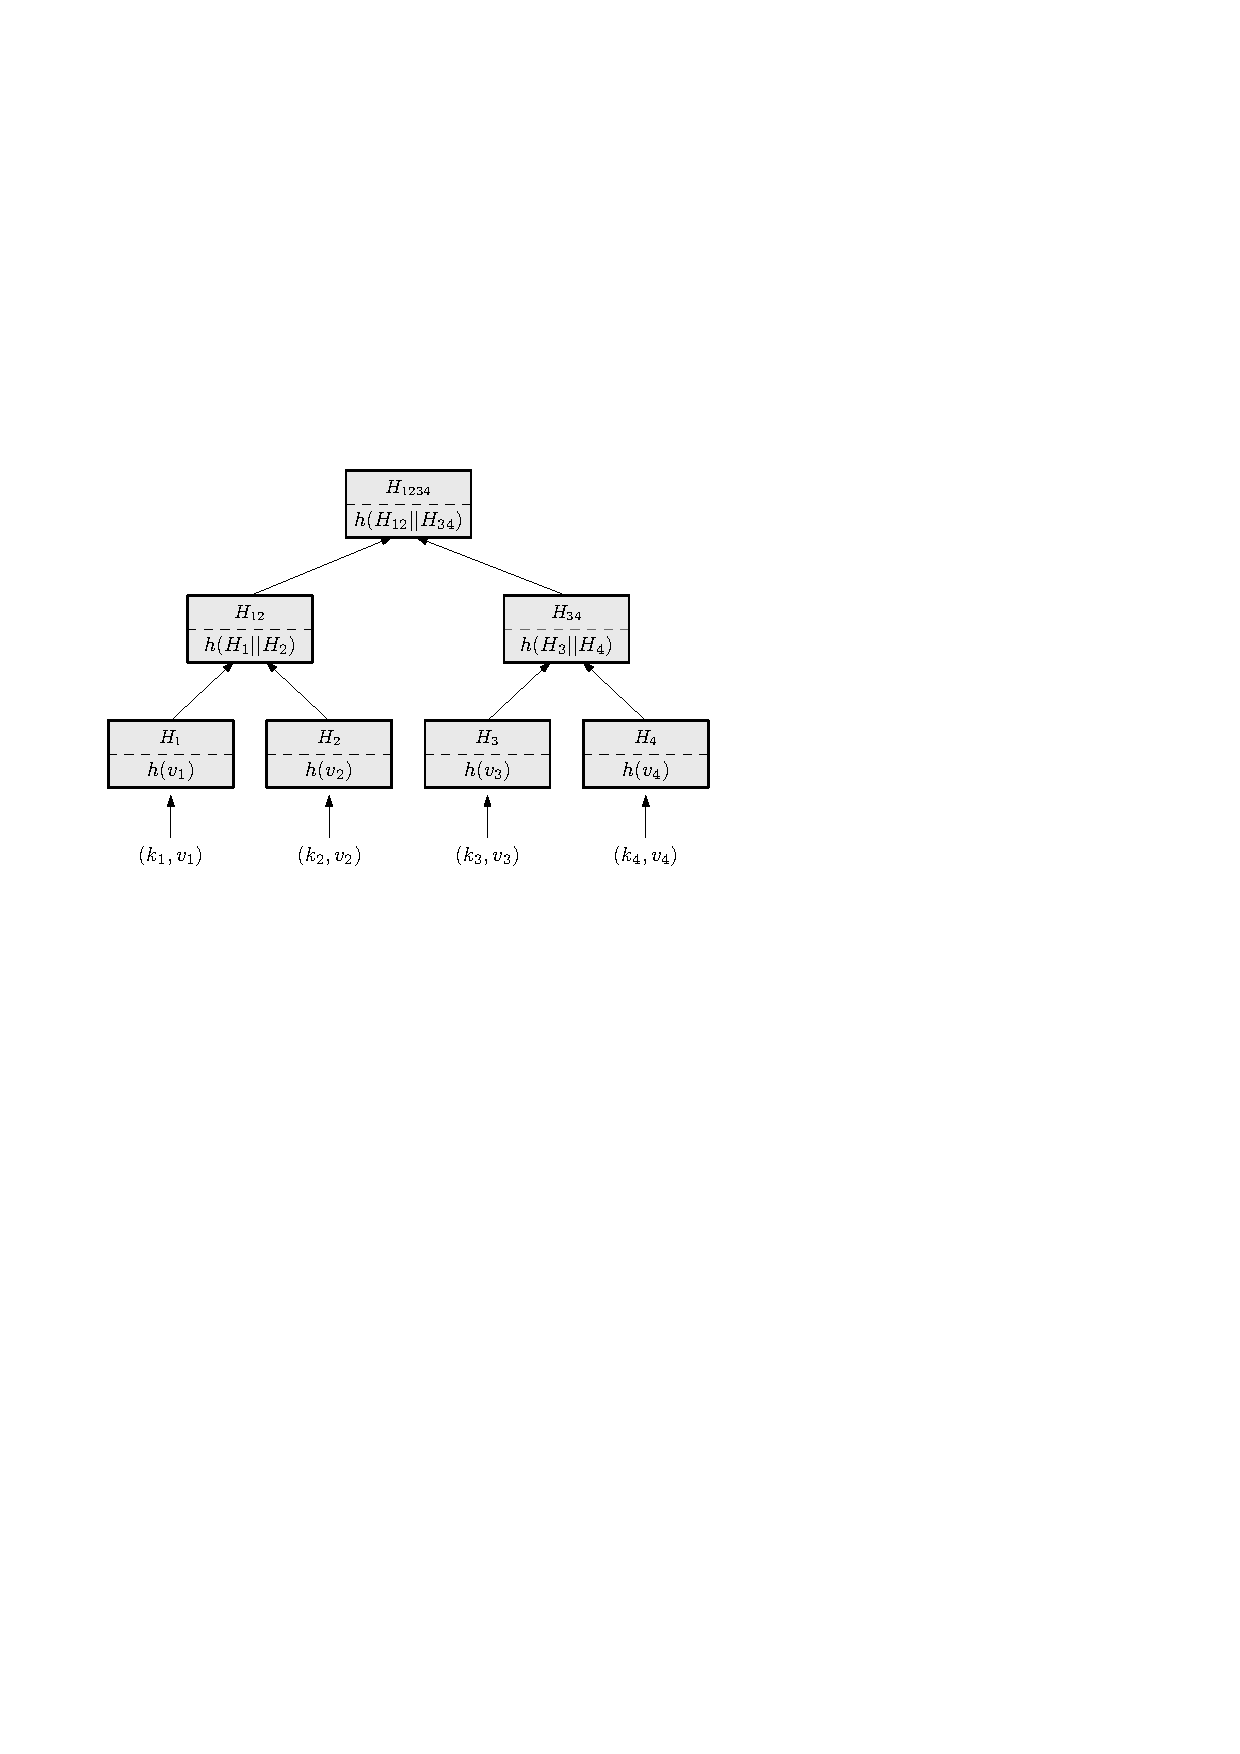
\includegraphics{img/capuno/mht.pdf}
	\caption{Un esempio di Merkle Tree. $h$ è la funzione di hash.}
	\label{fig:mht}
\end{figure}

Come ogni ADS, ad una richiesta \emph{T.get(k)}, dove si richiede il valore $v$ associato alla chiave $k$, si ottiene anche una \emph{proof} associata a $v$. La proof è una struttura dati utile a verificare l'integrità del valore a cui è associata. In particolare, in un Merkle Tree la proof si ottiene dall'Algoritmo~\ref{alg:proof}.

\begin{algorithm}
	\caption{Calcolo della proof in un MHT $T$ associata alla chiave $k$}
	\begin{algorithmic}
		\Procedure{get\_proof}{$k$}
			\State{Sia $n$ la foglia di $T$ associato a $k$}
			\State{$P \leftarrow [~]$}
			\While{$n.parent \neq T.root$}
				\If{$n.parent.right = n$}	\Comment{$n$ è un figlio destro}
					\State $Tag \leftarrow R$
					\State $h_f \leftarrow n.parent.left.value$
				\Else										\Comment{$n$ è un figlio sinistro}
					\State $Tag \leftarrow L$
					\State $h_f \leftarrow n.parent.right.value$
				\EndIf
				\State{$P.$\Call{append}{$(Tag, h_f)$}}
				\State{$n \leftarrow n.parent$}
			\EndWhile
			\Return $P$
		\EndProcedure
	\end{algorithmic}
	\label{alg:proof}
\end{algorithm}

La Figura~\ref{fig:mht_proof} mostra un esempio di proof, rappresentata dalla lista composta dai nodi grigi per il valore $v_5$. Considerato il cammino $p$ da $v_5$ al root, rappresentato in figura con una linea tratteggiata, si selezionano i nodi $H_6$, $H_{78}$ e $H_{1234}$, fratelli dei nodi percorsi in $p$. La proof risultante è quindi la lista di coppie $[(H_6, L), (H_{78}, L), (H_{1234}, R)]$.

\begin{figure}
	\centering
	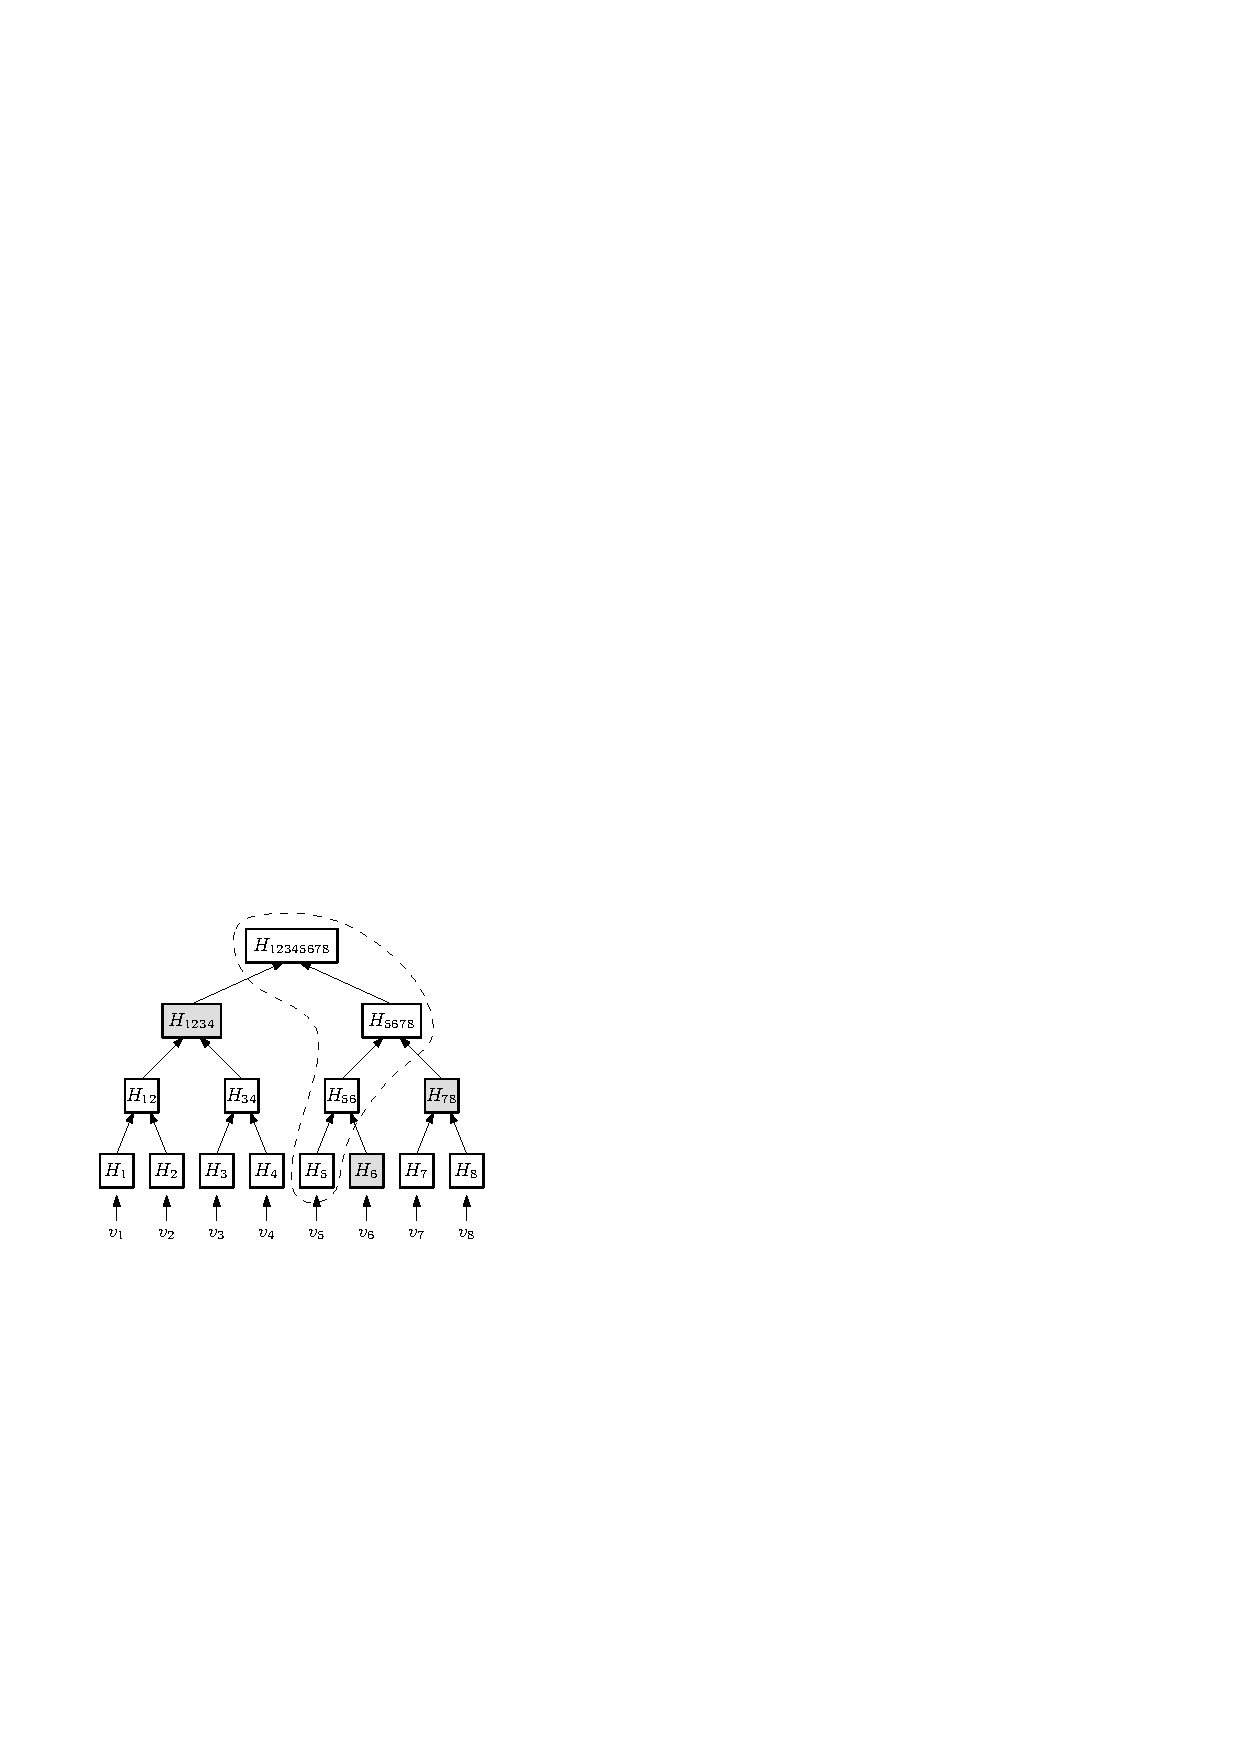
\includegraphics[scale=1.4]{img/capuno/proof.pdf}
	\caption{Proof di $v_5$ in un Merkle Tree. Essa è la lista composta dai nodi in grigio.}
	\label{fig:mht_proof}
\end{figure}

Un Merkle Tree utilizza uno spazio $O(|V|)$ e una dimensione della proof, un tempo per una query ed un tempo di verifica pari a $O(\log{|V|})$.

Un client possiede solo una copia locale del root-hash, mentre i dati sono su un server non fidato, ad esempio su cloud. Per verificare la veridicità del valore $v$ associato alla chiave $k$ ottenuto a seguito di una richiesta di \emph{get(k)} al server, il client calcola il root-hash dalla proof associata a $v$ e da $v$ stesso, con l'Algoritmo~\ref{alg:rh_proof}.

\begin{algorithm}
	\caption{Calcolo del root hash dalla proof}
	\begin{algorithmic}
		\Procedure{roothash\_from\_proof}{$p,v$}
			\State $h_1 = hash(v)$
			\State $L = len(p)$
			\For{$i \leftarrow 1$ to $L$}
				\State $Tag, h_{p_i} \leftarrow p[i]$
				\If{$Tag = R$}
					\State $h_{i+1} \leftarrow hash(h_{p_i} || h_i)$
				\Else
					\State $h_{i+1} \leftarrow hash(h_i || h_{p_i})$				
				\EndIf
			\EndFor
			\Return $h_L$
		\EndProcedure
	\end{algorithmic}
	\label{alg:rh_proof}
\end{algorithm}

La tecnica della \emph{potatura}~\cite{ponnapalli2019scalable}, o \emph{pruning}, consente di ridurre lo spazio occupato da un Merkle Tree, qualora non sia necessario rispondere a query su un certo insieme di chiavi, preservando la capacità di generare proof per le chiavi necessarie. Si ottiene rimuovendo le foglie non necessarie e lasciando gli hash delle radici dei sottoalberi al posto di esse. La Figura~\ref{fig:pruning} mostra un esempio di MHT potato.

\begin{figure}
	\centering
	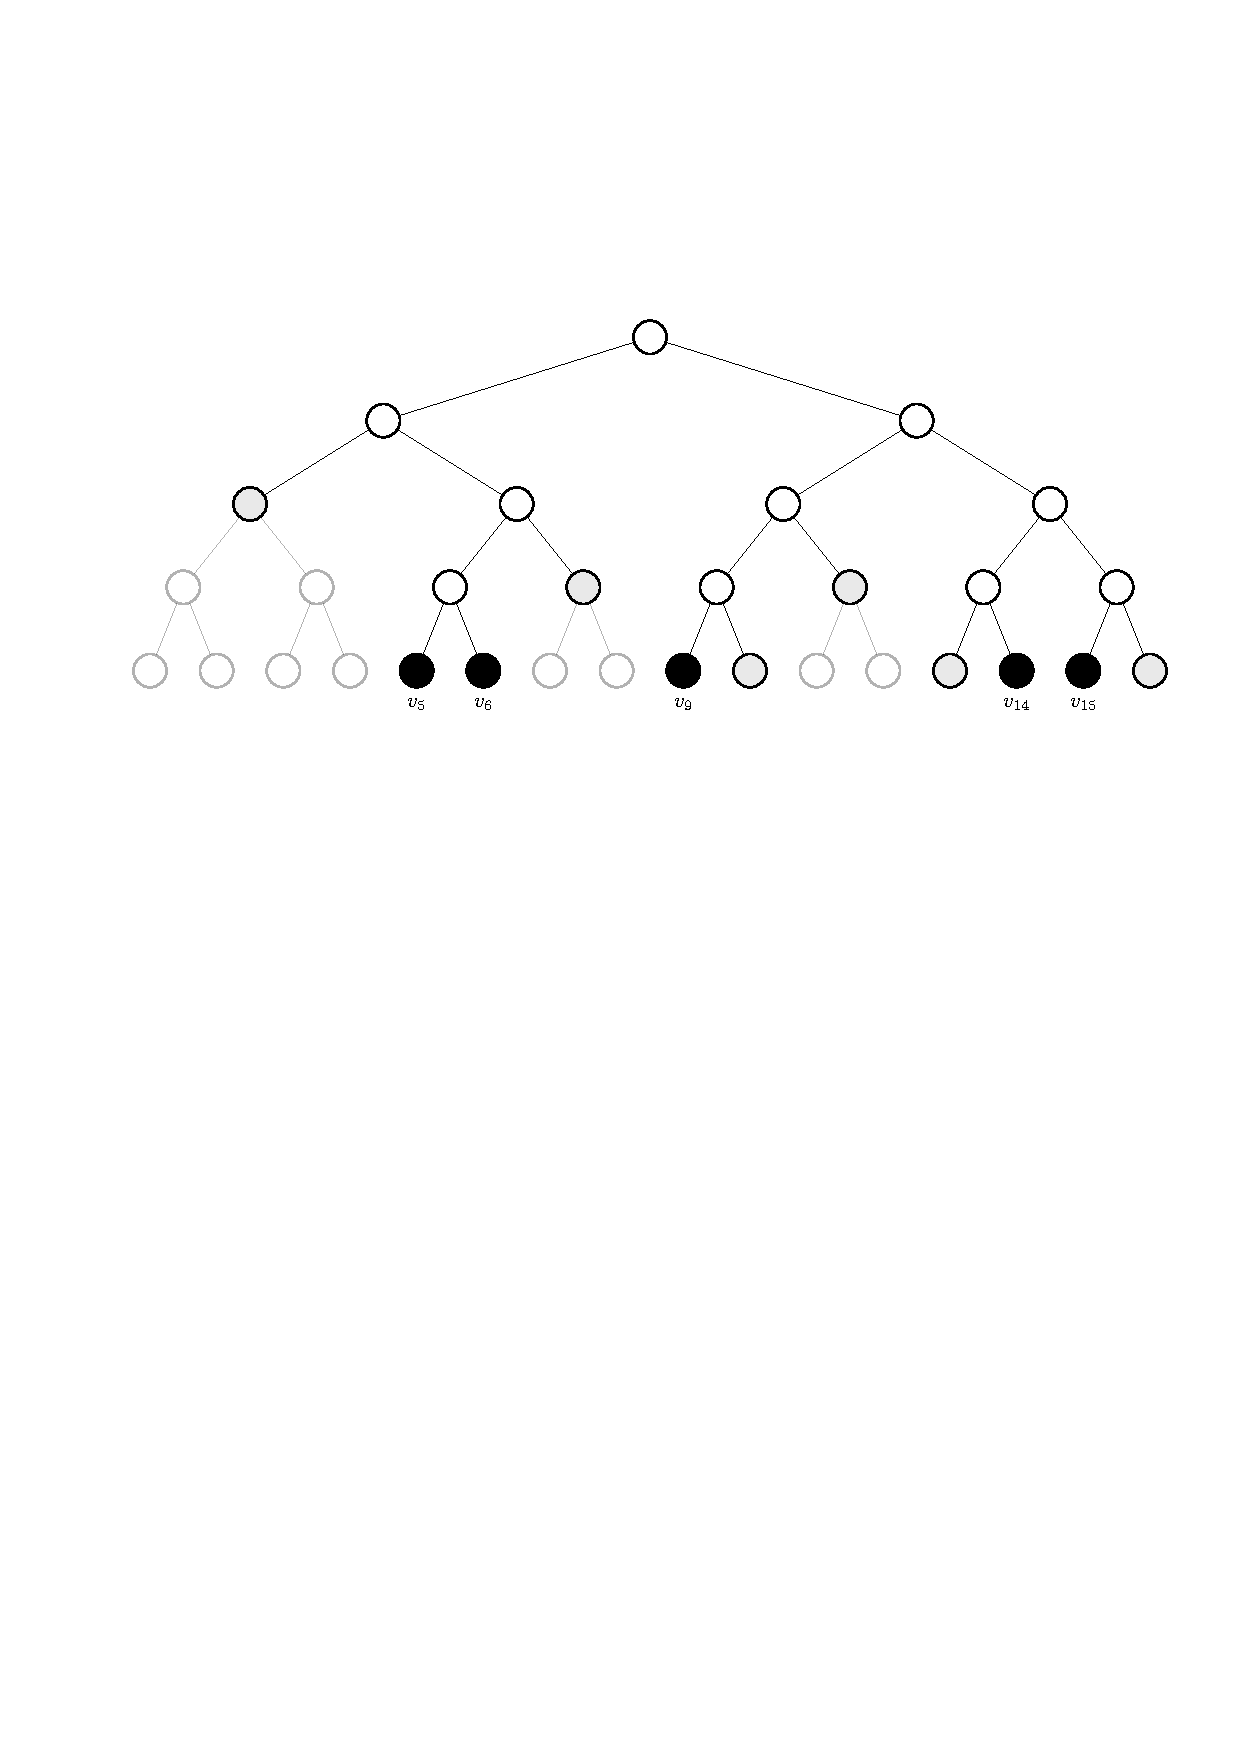
\includegraphics[scale=0.78]{img/capuno/pruned_mht.pdf}
	\caption{Esempio di Merkle Tree potato. Un nodo memorizza solo una parte dei valori ed i corrispettivi hash (nodi in nero), e le radici dei sottoalberi dei valori che non memorizza (nodi in grigio).}
	\label{fig:pruning}
\end{figure}

\section{Distributed Hash Table}

Una \textit{Distributed Hash Table} (\textit{DHT}) è un sistema di storage distribuito in grado di memorizzare dati sotto forma di coppie chiave-valore, in modo simile alle \emph{hash table}. Sono costruite su un \emph{keyspace}, ovvero l'insieme di tutte le chiavi, distribuite tra i nodi partecipanti. Se un nodo $n$ memorizza il valore $v$ associato alla chiave $k$, si dice che $n$ è \emph{autorità} per $k$. Molte implementazioni di DHT~\cite{maymounkov2002kademlia, ratnasamy2001scalable, stoica2001chord, zhao2004tapestry} permettono di effettuare un \emph{lookup}, l'operazione che consente di individuare il peer che detiene una certa risorsa, in modo efficiente, con un numero di scambi di messaggi e memoria dei peer sublineare, spesso $O(\log N)$, con $N$ il numero totale dei nodi della DHT (vedi Figura~\ref{fig:kademlia}).

\begin{figure}
	\centering
	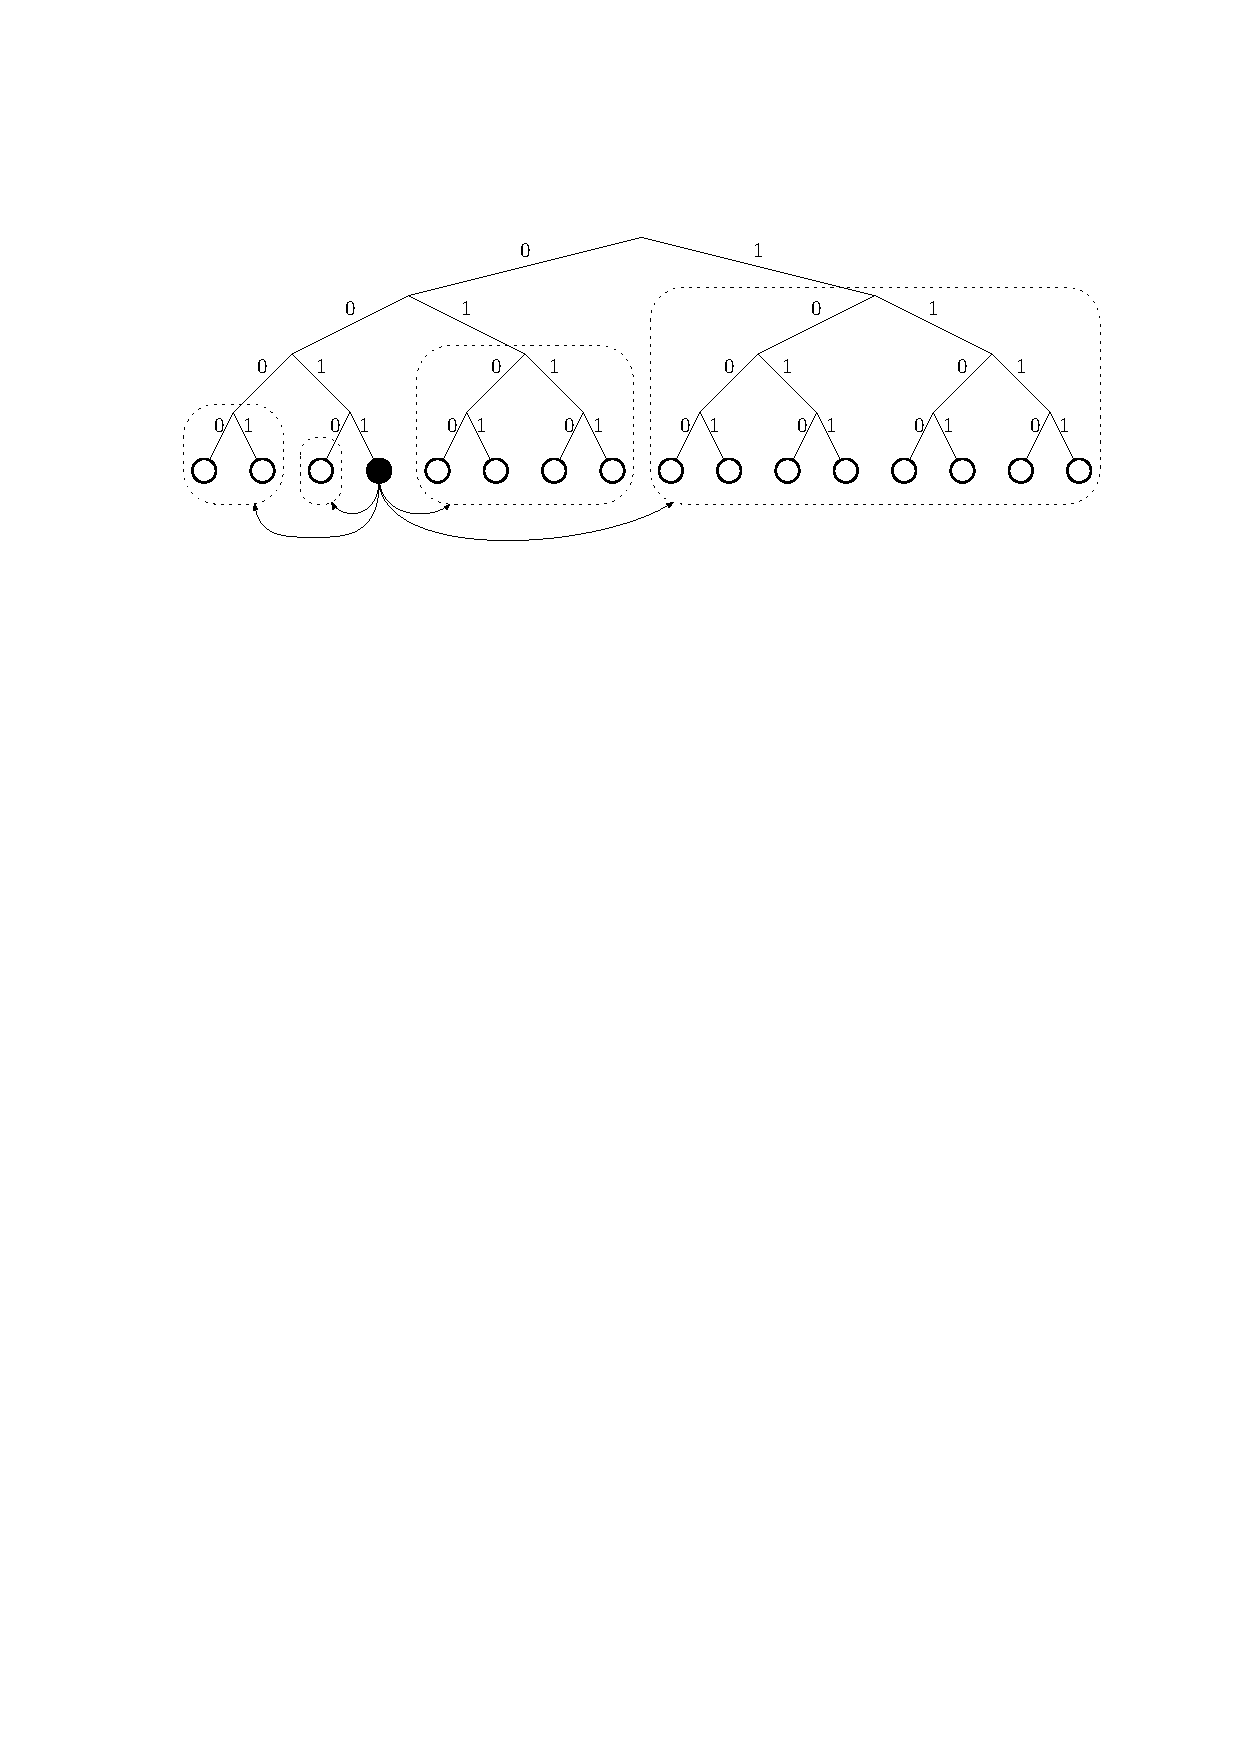
\includegraphics[scale=0.87]{img/capuno/kademlia.pdf}
	\caption{Rappresentazione della tabella di lookup di dimensione logaritmica rispetto al numero dei nodi in Kademlia.}
	\label{fig:kademlia}
\end{figure}

Una DHT presenta le seguenti proprietà:

\begin{itemize}
	\item[\cmark] \textbf{Decentralizzazione}: il sistema non ha alcun autorità centrale, ma ogni nodo è in grado di effettuare il lookup di una risorsa;
	\item[\cmark] \textbf{Scalabilità}: l'overhead di comunicazione e memoria dei peer pari a $O(\log N)$;
	\item[\cmark] \textbf{Tolleranza ai guasti}: il sistema è sempre disponibile anche se molti nodi si sconnettono o si guastano;
	\item[\cmark] \textbf{Efficacia}: una risorsa è sempre reperita se presente nel sistema.
	\item[\xmark] \textbf{Correttezza}: non esiste alcun modo per verificare che il dato ottenuto sia l'ultima versione memorizzata, o sia stata modificata dal peer autorità.
\end{itemize}

Per garantire la correttezza, si utilizzano le DHT \emph{autenticate}~\cite{tamassia2011efficient, bernardini2019blockchains}, in cui ogni nodo $n$ memorizza anche un'ADS potata, avente come foglie solo quelle per cui $n$ è autorità.
